\documentclass{subfiles}
\begin{document}

La teoria psicoanalitica di Freud descrive la personalità come composta da tre componenti 
interconnesse: l'\textbf{Es}, l'\textbf{Io} (o \textbf{Ego}) e il \textbf{Super-Io}. 
Questi tre elementi interagiscono tra loro e influenzano il comportamento e la 
psiche di un individuo. (Figura \ref{Modello Strutturale})


\begin{figure}[ht]
    \centering
    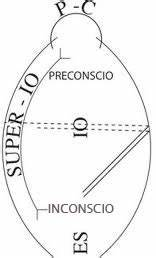
\includegraphics[width=0.2\linewidth]{ModellStrutturale.png}
    \caption{Modello Strutturale}
    \label{Modello Strutturale}
\end{figure}

\subsubsection{Es (Esistenza)}
L'\textbf{Es} è l'istanza originaria della personalità. Esiste sin dalla nascita e rappresenta 
gli aspetti ereditari, istintivi e primitivi della personalità

E' localizzato nell'\textbf{inconscio} e guida il comportamento umano secondo il 
\textbf{principio del piacere}. Questo principio afferma che i bisogni vanno soddisfatti 
immediatamente per evitare la tensione.

L'\textbf{Es} opera secondo il \textbf{processo primario}, cioè una modalità di funzionamento 
mentale tesa alla gratificazione immediata del desiderio.\\

\subsubsection{Io (Ego)}
L'\textbf{Io} deriva dall'\textbf{Es} ed è prevalentemente conscio e preconscio, sebbene sia 
in stretto collegamento con l'inconscio.

La sua funzione principale è quella di mediare tra le richieste dell'\textbf{Es}, le condizioni 
della realtà esterna e le norme sociali.

L'\textbf{Io} segue il \textbf{principio di realtà}, che implica prendere in considerazione la 
realtà esterna insieme agli impulsi e ai bisogni dell'\textbf{Es}. Valuta il rischio di 
soddisfare il bisogno e, se necessario, lo rimanda a quando le condizioni sono più favorevoli.

L'\textbf{Io} opera secondo il \textbf{processo secondario}, cioè secondo la capacità di 
dilazionare il soddisfacimento del desiderio fino a quanto le circostanze ambientali sono 
favorevoli.\\

\subsubsection{Super-Io}
Il \textbf{Super-Io} rappresenta il \textbf{`senso morale'} della personalità e incorpora i 
valori e le norme sociali interiorizzate dall'individuo.

Si forma attraverso il processo di internalizzazione delle regole genitoriali e sociali durante 
lo sviluppo dell'infanzia.

E' composto da due componenti principali : l'\textbf{Io ideale}, che si riferisce alle regole 
di buon comportamento o agli standard di eccellenza, e la \textbf{Coscienza}, che riguarda le 
norme e i comportamenti che i genitori disapprovano o puniscono.

Il \textbf{Super-Io} guida il comportamento morale e svolge un ruolo nella generazione di sensi 
di colpa quando l'individuo trasgredisce le norme sociali.\\

\subsubsection{Equilibrio tra Es, Io e Super-Io}
Quando le tre istanze, \textbf{Es}, \textbf{Io} e \textbf{Super-Io}, sono sviluppate, 
l'\textbf{Io} si trova costantemente coinvolto in un conflitto interno tra le richieste del 
\textbf{Es}, le esigenze della realtà esterna e le norme morali del \textbf{Super-Io}.

La capacità dell'\textbf{Io} di gestire questo conflitto è indicativa della sua \textbf{forza}. 
Un'\textbf{Io} con forza molto alta è in grado di gestire il conflitto in modo efficace, 
mentre un'\textbf{Io} con una forza bassa può essere sopraffatto dai conflitti interni, portando 
a un comportamento incoerente e alla lotta con emozioni contrastanti.\\

\end{document}